
\documentclass[draft,linenumbers]{agujournal}
\draftfalse
\journalname{Journal of Advances in Modeling Earth Systems (JAMES)}
\begin{document}


\title{Implementing plant hydraulics in the Community Land Model}
\authors{Daniel Kennedy\affil{1},
Sean Swenson\affil{2},
Keith Oleson\affil{2},
David Lawrence\affil{2},
Rosie Fisher\affil{2},
Pierre Gentine\affil{1}
}


\affiliation{1}{Columbia}
\affiliation{2}{NCAR}
\correspondingauthor{Daniel Kennedy}{djk2120@columbia.edu}

\begin{keypoints}
\item = enter point 1 here = 
\item = enter point 2 here = 
\item = enter point 3 here = 
\end{keypoints}


\begin{abstract}
= enter abstract here =
\end{abstract}

%====================
%  INTRODUCTION
%====================

\section{Introduction}



 - droughts are increasing 
      . \citep{cook2015}
      . \citep{dai2013}
      . amazon dry season lengthening \citep{fu2013}

 - vapor pressure deficit 
      . \citep{mcdowell2015}
      . \citep{novick2016b}
      . \citep{williams2013}

 - with lingering uncertainty in veg response
      . \citep{dekauwe2017}
      . \citep{friedlingstein2014}
      . \citep{anderegg2015b}


SPAC representation is important, defines:
  - vegetation water status
  - atmospheric carbon sink
  - hydrologic transpiration sink
  - magnitude and timing of transpiration

Representation in CLM is bad
  - also in other models
      . \citep{powell2013,ukkola2016}


Adds complexity, is it worth it, tractable?
       . hydraulic traits too hard \citep{drake2017}?, but people are doing it \citep{xu2016,christoffersen2016}

  - Trait information is available \citep{kattge2011,anderegg2015a} and valuable \citep{choat2012}
  - Water status information available \citep{konings2016,grant2016} and valuable \citep{momen2017,konings2017b}
  - Model structural information
  
Our goal:
  - parsimonious plant hydraulic implementation
  - setting a framework to represent vegetation water status
       . opening an interface to trait data, satellite VOD \citep{momen2017}
       . improving functionality

%====================
%  MODEL DESCRIPTION
%====================
\section{Model Description}

%Photosynthesis
\subsection{Photosynthesis}
\label{sect:A}
    The CLM5 photosynthesis model is largely inherited from CLM4.5 as described in \citet{bonan2011}, \citet{thornton2007},
    and \citet{oleson2013}.Photosynthesis is defined in three regimes: Rubisco-limited, light-limited, and export-limited 
    following \citet{farquhar1980} and \citet{harley1992}.The implementation extends \citet{sellers1996a,sellers1996b} with 
    colimitation following \citet{collatz1991}. 
    
    CLM5 photosynthesis is a two-big-leaf model, with a sunlit and shaded leaf per PFT per gridcell \citep{thornton2007, 
    dai2004, oleson2013}. The canopy fluxes module iterates for leaf surface energy balance.
    Within this, the photosynthesis module iterates to solve for intercellular CO$_2$ concentration, balancing stomatal flux of 
    CO2 with photosynthetic assimilation flux of CO2.
    
    Vegetation water stress is implemented via the vegetation water stress factor ($f_w$, dimensionless, 0 to 1, formerly 
    $\beta_t$). This factor multiplies the rate of maximum carboxylation ($V_{\text{cmax}}$) and the minimum stomatal 
    conductance ($g_0$) as described in \citet{oleson2013} and first implemented in \citet{sellers1996a,sellers1996b}. 
    
    With PHS, $f_w$ replaces the CLM4.5 transpiration beta function ($\beta_t$). 
    These factors are used by the photosynthesis model in the same way, but calculated differently. 
    The parameterization for $f_w$ is based on leaf water potential. 
    For $\beta_t$, the parameterization is based on soil water potential.
    The switch to leaf water potential adopts the framework where optimal stomatal conductance is concurrently limited by hydraulic constraints \citep{novick2016a}


%Stomatal Conductance
\subsection{Stomatal Conductance}
\label{sect:gs}
    CLM5 uses the Medlyn stomatal conductance model, which reconciles the empirical and optimal approaches to modeling 
    stomatal conductance \citep{medlyn2011}. 
    Stomatal conductance of CO2 is related to net photosynthesis ($A_n$), atmospheric CO2 concentration at the leaf surface 
    ($C_a$), and the square root of the vapor pressure deficit near the leaf surface ($\sqrt{D}$).
    \begin{equation}
    g_s=g_0+\left(1+\dfrac{g_1}{\sqrt{D}}\right)\dfrac{A}{C_a}
    \end{equation}
    The model features two parameters $g_0$ ($\mu$mol / m2 / s) and $g_1$ (kPa$^{0.5}$). The $g_0$ parameter fits a 
    minimum stomatal conductance. The $g_1$ parameter relates to the water cost guiding the optimization of carbon 
    assimilation.
    
    The attenuation of stomatal conductance due to water stress follows the CLM4.5 formulation as described in 
    \citet{oleson2013} and \citet{bonan2011}. Prognostic water stress ($f_w$, ranging from 0-1) attenuates stomatal 
    conductance directly via multiplication of $g_0$, and indirectly via multiplication of $V_{\text{cmax}}$. 
    
    What did \citet{zhou2014} show? What did \citet{manzoni2011} show? Can we cite changge?

% Plant Hydaulics
\subsection{Plant Hydraulic Stress (PHS)}
  We implemented a simplified plant hydraulic framework in CLM. 
  We used hydraulic laws and the corresponding circuit analogy to represent the 
  flow of water through the soil-plant-atmosphere continuum. 
  The hydraulic framework is used to effect water stress associated with increasing xylem tension
  and for calculating the layer-by-layer soil transpiration sink. 
  Water stress attenuation of transpiration and photosynthesis is based on prognostic leaf water potential. 
  We refer to the module that cranks out the hydraulic solution as Plant Hydraulic Stress (PHS).
  During model development, design decisions followed a preference for a simplified implementation that,
  whenever possible, conformed to existing CLM architecture.
  
  \begin{figure}[h]
     \centering
     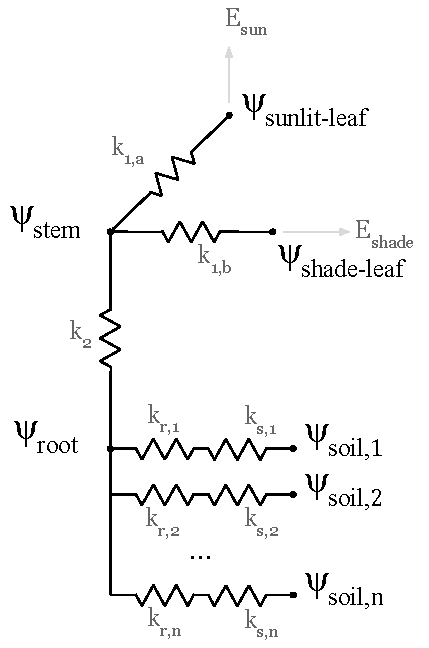
\includegraphics[width=9pc]{../figs/circuit.pdf}
     \caption{Plant hydraulic circuit analog schematic}
     \label{circuit}
  \end{figure}

%Hydraulic schematic and segmentation
  \subsubsection{Hydraulic schematic and segmentation}
  PHS solves for the set of vegetation water potential values 
  ($\psi_{\text{root}}$, $\psi_{\text{stem}}$, $\psi_{\text{shade-leaf}}$, $\psi_{\text{sun-leaf}}$ ) 
  that matches water supply (root water uptake) to water demand (transpiration), 
  while maintaining continuity of water flow throughout the soil-plant-atmosphere continuum.
  The PHS circuit analogy is presented in Figure \ref{circuit}.
  At each node, we resolve water potential, and, between nodes, we resolve the flux of water.
  The resistors define the segment conductance to water. 
  The segmentation is designed to take advantage of field-measured hydraulic traits 
  and to conform to the existing CLM architecture.
  From CLM, we inherit the vertically discretized soil layers and the two-layer (sunlit vs. shaded) canopy.
  From the hydraulic theory, we additionally segment the resistance across the soil matrix from the 
  resistance through root tissue \citep{williams1996}. 
  Likewise we segment the resistances through the root, stem, and leaf tissue to allow for differences
  in their parameterizations \citep{simonin2015, sperry2015}.

%Water Supply
    \subsubsection{Water supply}
    \label{sect:supply}
    Water supply is modeled via hydraulic laws where flow is proportional to the gradient in water potential. 
    Flow of water ($q$) is the product of the path hydraulic conductance ($k$) and 
    the gradient in water potential (accounting for change in gravitational potential). 
    Equation \ref{eq:darcy} represents the flow from node 1 to node 2. 
    
     \begin{linenomath*}
     \begin{equation}
     \label{eq:darcy}
     q = k\left(\psi_1 - \psi_2 - \rho g \Delta z\right)
     \end{equation}
     \end{linenomath*}
    
    PHS does not include plant tissue water storage (by circuit analogy: capacitance). 
    Capacitance significantly complicates the water potential solution \citep{celia1990}
    and is challenging to parameterize \citep{bartlett2016}.
    However, buffering of water stress provided by tissue water storage can be important
    especially on sub-daily timescales \citep{meinzer2009}, whereby its inclusion may be warranted 
    in future model generations.

     
     Vegetation segment conductance is modeled with empirical xylem vulnerability curves \citep{tyree1989}, 
     where segments lose conductance with increasing drought status associated with 
     cavitation and embolism \citep{holbrook2001}.
     The vulnerability curves model loss of conductance relative to maximum conductance using two parameters: 
     $c_k$, a sigmoidal shape-fitting parameter, and 
     $p_{50}$, the water potential at 50\% loss of segment conductance (following \cite{gentine2016}). 
     These parameters can be estimated from field experiments \citep{sack2002}, 
     and $p_{50}$ is available in the TRY trait database \citep{kattge2011}.
     Parameterization based on $p_{50}$ is especially attractive in light of the call for transition to
     a trait-based model paradigm \citep{anderegg2015a}.
     The loss of xylem conductivity is based on lower terminus water potential ($\psi_1$)
     as is typical in other models \citep{xu2016}, but 
     may underestimate the integrated loss of conductivity \citep{sperry2015}. 
         
     \begin{linenomath*}
     \begin{equation}
     \label{eq:vulnerability}
     k = k_{\text{max}} \, 2^{-\left(\dfrac{\psi_1}{p_{50}}\right)^{c_k}}
     \end{equation}
     \end{linenomath*}
     
     PHS models root, stem, and leaf conductances according to equation \ref{eq:vulnerability}.
     The parameterization of $k_{\text{max}}$ varies by hydraulic segment (see details in Appendix zqz).
     The conductance across the matrix from soil to root follows \citet{williams2001} and \citet{bonan2014} 
     to estimate the distance between roots for the length-scaling of soil conductance. 
     Bulk soil resistivity is based on \citet{clapp1978} as described in \citet{oleson2013}.
    
%Water demand
    \subsubsection{Water demand}
    
    Water demand is based on the Medlyn stomatal conductance model (see section \ref{sect:gs}), 
    which we adjust for water stress with $f_w$, the PHS water stress factor. 
    The water stress factor multiplies $V_{\text{cmax}}$ and minimum stomatal conductance $g_0$.
    We calculate the water stress factor based on leaf water potential, such that 
    as leaf water potentials decrease, stress increases.
    The PHS stress factor is the same as the CLM4.5 stress function in that, once calculated, they are used
    to attenuate photosynthesis and stomatal conductance in the same way.
    The PHS stress factor is different from (and better than) the CLM4.5 stress function, because that one 
    is calculated based on soil potential.
    
     \begin{linenomath*}
     \begin{eqnarray}
     \begin{aligned}
     \label{eq:demand}
     E_{\text{sun}}     &= E_{\text{sun,max}} \, 2^{-\left(\dfrac{\psi_{\text{sun-leaf}}}{\psi_{50}}\right)^{c_k}} \\
     E_{\text{shade}} &= E_{\text{shade,max}} \, 2^{-\left(\dfrac{\psi_{\text{shade-leaf}}}{\psi_{50}}\right)^{c_k}}
     \end{aligned}
     \end{eqnarray}
     \end{linenomath*}
    
    
     \begin{linenomath*}
     \begin{eqnarray}
     \begin{aligned}
     \label{eq:stress}
     f_{\text{w,sun}}         &= \dfrac{g_{\text{s,sun}}}{g_{\text{s,sun,max}}} \\
     f_{\text{w,shade}}     &= \dfrac{g_{\text{s,shade}}}{g_{\text{s,shade,max}}} \\
     \end{aligned}
     \end{eqnarray}
     \end{linenomath*}
    

     
    We define $f_w$ as the ratio of stressed to unstressed stomatal conductance (Equation \ref{eq:stress}).
    The unstressed stomatal conductance is the stomatal conductance when calculated with $f_w=1$
    (i.e. without water stress). 
    The "stressed" stomatal conductance is the stomatal conductance associated with the PHS module
    water flow solution, which matches vegetation water supply with vegetation water demand 
    (Section \ref{sect:solution}).
    This solution is the set of vegetation water potentials ($\psi$) where water supply
    (a generally increasing function of $\left|\psi\right|$) matches water demand
    (a generally decreasing function of $\left|\psi\right|$).
    The decrease of water demand at lower potentials is modeled with a two-parameter sigmoidal function 
     applied to maximum transpiration (Equation \ref{eq:demand}). 
     The parameters are $\psi_{50}$, the leaf water potential at 50\% loss of transpiration and 
     $c_k$ a sigmoidal shape-fitting parameter.
     
     Whereas the water supply parameters (see Section \ref{sect:supply}) 
     relate to hydraulic traits often measured in the field, 
     the hydraulic demand parameters $\psi_{50}$ and $c_k$ reflect the emergent property of stomatal control
     and must be empirically derived. 
     Likewise CLM4.5 had two empirical stomatal control parameters, which were the soil matric potentials 
     corresponding to stomates fully closed and stomates fully open (see Section \ref{sect:btran}).
     The functional form of stomatal control is not generally agreed upon, and as such, 
     should be investigated farther. Recent modeling studies suggest sperry,xu,christo.

%PHS solution
    \subsubsection{PHS solution}
    \label{sect:solution}
    
    PHS solves for the set of vegetation water potential values ($\psi$) that matches water supply
    (root water uptake) to water demand (transpiration), while satisfying continuity across the four water flow
    segments (soil-to-root, root-to-stem, stem-to-leaf, and leaf-to-transpiration). 
    We compute the flux divergence $f$ (representing the mismatch of flow in and out of each segment)
    for a given set of vegetation water potential values $\psi_i$, and iteratively update $\psi$ until $f\to0$.
    
    \begin{linenomath*}
    \begin{equation} 
    \psi = \left[
    \begin{array}{c}
    \psi_{\text{sun}} \\ 
    \psi_{\text{shade}} \\ 
    \psi_{\text{stem}} \\ 
    \psi_{\text{root}}            
    \end{array} \right]
    \end{equation}
    \end{linenomath*}
    
    \begin{linenomath*}
    \begin{equation}
    f\left(\psi\right) = \left[ 
    \begin{array}{c}
    E_{sun}-q_{sun}\\
    E_{shade}-q_{shade}\\
    q_{sun}+q_{shade}-q_{stem}\\
    q_{stem}-\sum_{j=1}^n{q_{root,j}}
    \end{array} \right]
    \end{equation}
    \end{linenomath*}
    
    \begin{linenomath*}
    \begin{equation}
    A = \dfrac{df}{d\psi}
    \end{equation}
    \end{linenomath*}    
    
    While $\left|f\right|>0$
    \begin{linenomath*}
    \begin{equation} \begin{aligned}
    \label{eq:iter}
    \Delta\psi &=A^{-1}f\left(\psi_i\right) \\
    \psi_{i+1}  &= \psi_i + \Delta\psi
    \end{aligned} \end{equation}
    \end{linenomath*}    
    
    The numerics are especially tractable because $f$ has analytical derivatives and $A$ 
    (a 4x4 matrix with six null entries) is easily inverted when well-conditioned. 
    Supply and demand converge, because transpiration demand decreases with more negative 
    leaf water potentials and supply increases with more negative leaf water potentials.
    
    Furthermore several simplifications were made that decreases the numerical complexity.
    For the purposes of the PHS solution, soil potentials are assumed constant during each timestep.
    During each PHS iteration (\ref{eq:iter}), transpiration is assumed to be linear with $f_w$,
    which precludes updating leaf temperature and intercellular CO$_2$.
    Plant tissue water storage (capacitance) is not represented, whereby the solution does not
    depend on the previous timestep and has no time derivatives.

%====================
%  EXP DESCRIPTION
%====================
\section{Experiment Description}
    
    
    
%====================
%  BTRAN
%====================

\section{BTRAN}
\label{sect:btran}
    PHS replaces the transpiration beta function ($\beta_t$, colloquially btran), 
    which is the phenomenological soil water stress function in CLM4.5,
    as described in \citet{oleson2013,sellers1996a,sellers1996b}.
    
    Recent studies suggest that the $\beta_t$ parameterization introduces model bias in turbulent fluxes \citep{bonan2014}
    and contributes to unrealistic drought response of photosynthesis and stomatal conductance  \citep{powell2013}.
    Furthermore, if $\beta_t$ represents a plant hydraulic safety mechanism, attenuating stomatal conductance to avoid
    dangerously low leaf water potentials, it makes sense to represent more of the hydraulic architecture (a la SPA or PHS)
    and assess hydraulic safety based on prognostic leaf water potential.
    
    But weirdly, this isn't even the biggest home run for why to replace btran. Because btran, while responsible for applying
    water stress to photosynthesis, also sets the framework for vegetation root water extraction. And it does a terrible job!
    In this section, we recast the btran soil water extraction equations into a hydraulic framework, for comparison to the PHS implementation, making the case that this is a good reason to ditch btran.
    
    Btran is unitless, ranging from 0 to 1, with 1 corresponding to no water stress, and 0 corresponding to fully water stressed. 
    Btran is calculated based on a root-fraction weighted average of soil layer wilting factor ($w_i$), which is a bounded linear 
    function of soil water potential ($\psi_i$) relative to PFT parameters defining the soil potential with stomates fully open ($
    \psi_{fo}$) and fully closed ($\psi_{fc}$). Note that root fraction ($r_i$) must sum to 1.
    
    \begin{linenomath*}
    \begin{equation} \beta_t = \sum_{i=1}^{n}{r_iw_i}
    \end{equation}
    \begin{equation} 
    \label{bt:2}
    w_i=0 \leq \dfrac{\psi_i-\psi_{fc}}{\psi_{fo}-\psi_{fc}} \leq 1
    \end{equation}
    \end{linenomath*}
    
    CLM4.5 uses $\beta_t$ to attenuate photosynthesis and stomatal conductance with soil water stress. It is also used for 
    modeling vegetation water extraction from the soil column. The total transpiration ($T$) is partitioned among the soil layers, 
    based on the $\beta_t$ framework of soil water availability. For each soil layer ($i$), the flux to transpiration ($q_i$) is 
    calculated as the layer root fraction times the layer wilting factor, normalized by $\beta_t$. This guarantees that the total 
    soil water extraction equals the transpiration.
    \begin{linenomath*}
    \begin{equation}
    \label{bt:4}
    q_i = \dfrac{r_i w_i}{\beta_t}T
    \end{equation}
    \end{linenomath*}
    
    The PHS implementation adopts the hydraulic framework for soil water extraction, where the flux to transpiration ($q_i$) is 
    the product of the hydraulic conductance ($k$), the area basis of that conductance ($A$), and the gradient in water 
    potential driving the flow ($\Delta\psi$).
    \begin{linenomath*}
    \begin{equation}
    q_i = kA\Delta\psi
    \end{equation}
    \end{linenomath*}
    
    With some manipulation, we can recast (\ref{bt:4}) into the hydraulic framework. Define $T_{\text{max}}$, such that: $T = 
    \beta_t T_{\text{max}}$ and use this expression to replace $T$ in (\ref{bt:4}).  Likewise replace $w_i$ in (\ref{bt:4}) with the 
    formula from (\ref{bt:2}).
    
    \begin{linenomath*}
    \begin{equation} 
    q_i = \dfrac{T_{\text{max}}}{\psi_{fo}-\psi_{fc}} r_i \left(\psi_i-\psi_{fc} \right)
    \end{equation}
    \end{linenomath*}
    
    This yields Btran analogs for the three terms of $q_i = kA\Delta\psi$
    \begin{linenomath*}
    \begin{equation} \begin{aligned}
    k &= \dfrac{T_{max}}{\psi_{fo}-\psi_{fc}} \\
    A &= r_i \\
    \Delta\psi &= \psi_i - \psi_{fc} \\
    \mbox{constrained by:} \qquad
    \Delta\psi &=
    \begin{cases}
    0                          & \text{if } \psi_i<\psi_{fc}  \\
    \psi_{fo}-\psi_{fc} & \text{if } \psi_i>\psi_{fo}
    \end{cases}
    \end{aligned}\end{equation}
    \end{linenomath*}
    
    Issues: \\
    1) No gravity component \\
    2) No length-scaling of conductance \\
    3) No dependence on absolute root biomass \\
    4) Constant pulling $\psi$ \\
    5) Would like to represent reverse flows \\
    
\section{Results and Discussion}
\subsection{Modeling vegetation water potential}

Both cases: stem, sunlit, shaded basically indistinguishable, 3 lines overlap. \\
Ambient Midday (1pm): -1.95, -1.94, -1.93 \\
TFE Midday (1pm): -2.29, -2.28, -2.27 \\

Ambient: Predawn (5am) root water potential = -0.07MPa \\
TFE: Predawn (5am) root water potential = -0.28MPa \\
delta = -0.22 MPa

Ambient: Midday (1pm) root water potential = -0.10 MPa, for a drop of 0.03 MPa relative to predawn \\
TFE: Midday (1pm) root water potential = -0.60 MPa, for a drop of 0.32 MPa relative to predawn \\
delta = -0.28 MPa

Ambient: Midday (1pm) sun leaf water potential = -1.95 MPa, for a drop of 1.85 MPa relative to midday roots \\
TFE: Midday (1pm) sun leaf water potential = -2.29 MPa, for a drop of 1.69 MPa relative to midday roots \\
delta = +0.16 MPa

Discussion:
Overlapping lines tips hand on naive approach, likewise instant refilling.
Water potential values are in range (cite).
LWP drop due to TFE is -0.34MPa, probably small.
Due in equal measure to change in predawn water potential (-0.22 MPa) and change in soil-to-root drop (-0.28 MPa). 
Stem drop actually attenuated (+0.16 MPa).
Stem drop smaller because though PLC increases, transpiration decreases to larger effect.
Consistent with findings that root resistance is most important in Amazonia (rosie).

\subsection{Stress function}

Monthly means

Ambient \\
PHS-off has no stress. PHS-on has significant stress, ranging from 0.6 to 0.9.
PHS-on stress has a seasonal cycle, least stress in February, most stress in September.
Predawn water potential annual change less than 0.1 MPa
Instead seasonality due to transpiration demand, driven by solar radiation and VPD. \\
As a result, PHS-on has less GPP than off, and less seasonality in GPP. Likewise for transpiration.

TFE \\
In both cases, the effect of TFE accumulates through the simulation. 
The effect of TFE is underestimated in both cases, seeming to overestimate the ability of soil water to buffer stress.
For PHS-on, the effect of TFE is small, with additive stress peaking in November: adding 12\% to the stress in Nov-2002 and 19\% to the stress in Nov-2003.
For PHS-off, the effect of TFE is larger, adding 45\% in January 2003  and 75\% in December 2003. \\
Note the different seasonality
PHS-on has the most stress in JAS and least stress in JFM. 
PHS-off has the most stress in DJF and least stress in JJA. \\

PHS-off stress is driven by soil potential (weighted by root fraction), leading to no stress in the ambient conditions.
Likewise with TFE, soil potential doesn't rebound until well into the wet season, whereby stress peaks in DJF.

PHS-on stress is a function of leaf water potential, which responds to both soil potential and atmospheric demand. 
Ambient dynamics of predawn root water potential are 0.1 MPa corresponds to about 2-3\% extra stress, without factoring in lost conductance
Ambient dynamics of stress are about 30\%. Mostly due to atmospheric demand.

TFE causes 2003 SON predawn water potential to decrease by 0.22MPa. 
Added stress is due to soil forcing, but still depends on atmospheric demand, 
because lowering water potential is more damaging during the dry season,
due to nonlinear stress function.

Diurnal cycle

Another look at PHS-on has significant stress in ambient, PHS-off does not.
TFE has a larger effect on PHS-off lowering stress function by about 50\%.
PHS-on TFE adds about 15\% to midday stress.

PHS-on introduces diurnal cycle to stress function, responding to atmospheric demand, peaking after noon
when VPD and solar radiation are high. 

The PHS-on stress function deviates from 1 to limit photosynthesis and transpiration when the unattenuated Medlyn transpiration requires
very negative leaf water potential. At night, this is typically not the case, so the stress function evaluates to 1. 
A time-average of the stress function is not appropriate for interpreting the effect of water stress on photosynthesis.
In this case, the time averages of the stress function over SON 2013 are 0.94,0.88,1,0.52
The average photosynthesis values are 8.1,7.3,9.1,6.2 g/m2/d
Very helpfully, we can use the phs-off, amb as maximal photosynthesis. Divide all the averages by that you get
0.89,0.8,1,0.68.
TFE PHS-off GPP is 68\%, which is higher than the stress function of 52\%.
Why? Because though stress increases, WUE also increases, because with lower stomatal conductance, C$_i$ increases.
PHS-on GPP is 89\% and 80\%, which are lower than the time average stress functions.
Why? Because all the ones at night, shouldn't count.

Instead we should look at the inner product of stress with a notion of potential photosynthesis (in this case PHS-off, AMB) divided by total potential photosynthesis.
This weighted average stress function over SON2013 is 0.84,0.71,1,0.53, delivering a more consistent metric for average stress, robust to diurnal variation.

Stress vs. VPD

PHS-on introduces a diurnal course to the water stress function, with plants experience more stress near midday. This relationship is a function of transpiration demand, driven by solar radiation and VPD. In figure \ref{fig5}, the effect of high VPD is shown for the four experiments. Data are constrained to timesteps with downwelling solar radiation between 400 and 425 W/m$^2$ (n=775), to highlight the VPD effect. Data are colored based on the soil moisture state. For PHS-on, soil moisture state is predawn root water potential. For PHS-off, soil moisture state is root-fraction weighted soil matric potential. The data are split into terciles, coloring the driest tercile red, the wettest tercile blue, and the intermediate tercile yellow.

For PHS-off there's no stress in the ambient simulation. 
With TFE there is significant stress, with a strong relationship to soil potential, and no relationship with VPD. 

For PHS-on there is stress in the ambient simulation, with more stress with increasing VPD
and no strong relationship between stress and soil state.
With TFE stress increases, and in this case, drier soil states are clearly related to increased stress.

For PHS on, stress is imposed to constrain the unattenuated transpiration based on leaf water potential. 
As leaf water potential becomes more negative, the stress function evaluates lower, attenuating photosynthesis and transpiration.
This provides a hydraulic safety constraint to the GPP and transpiration solutions.
PHS functionality is as expected in these simulations, where hydraulic danger can derive from both high atmospheric demand and drying soils.
In the ambient simulation, with well-watered conditions, hydraulic danger is present, but only due to atmospheric demand. 
With TFE, hydraulic danger is imposed by both high atmospheric demand and dry soils.

\subsection{Hydraulic redistribution}

\subsection{Extraction via hydraulic gradient}
deep roots \citep{nepstad1994}

\subsection{Soil profile}

For phs-off, root-area averaged smp, for SON 2003, ambient throughfall is -0.04 MPa.
With TFE, this decreases to -1.39 MPa. Much bigger drop than in phs-on, -0.07 to -0.28MPa.

Cumulative ET, \\
phs on, amb = 4.26 m \\
phs on, tfe = 4.16 m \\
phs off, amb = 4.53 m \\
phs off, tfe = 4.31 m \\

For comparison, total precip is 6.7 meters and precip during TFE is 4.4 meters,
whereby TFE is delta of approximately 2 meters of water.



    
\clearpage    

\section{Figures}
  \begin{figure}[h]
     \centering
     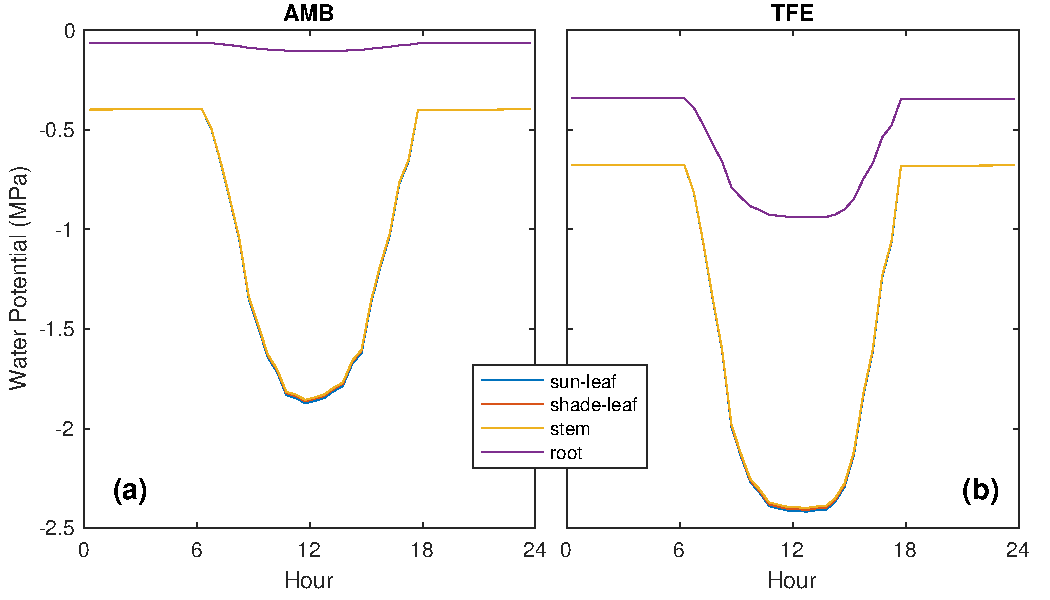
\includegraphics[width=30pc]{../figs/fig2.pdf}
     \caption{Diurnal mean root, stem, shaded leaf, and sunlit leaf water potentials for 2003 dry season (SON), Caxiuan\~a national forest, Brazil.
     (a) Ambient throughfall conditions (b) 50\% throughfall excluded
     }
     \label{fig2}
  \end{figure}
  
  \clearpage   
  \begin{figure}[h]
     \centering
     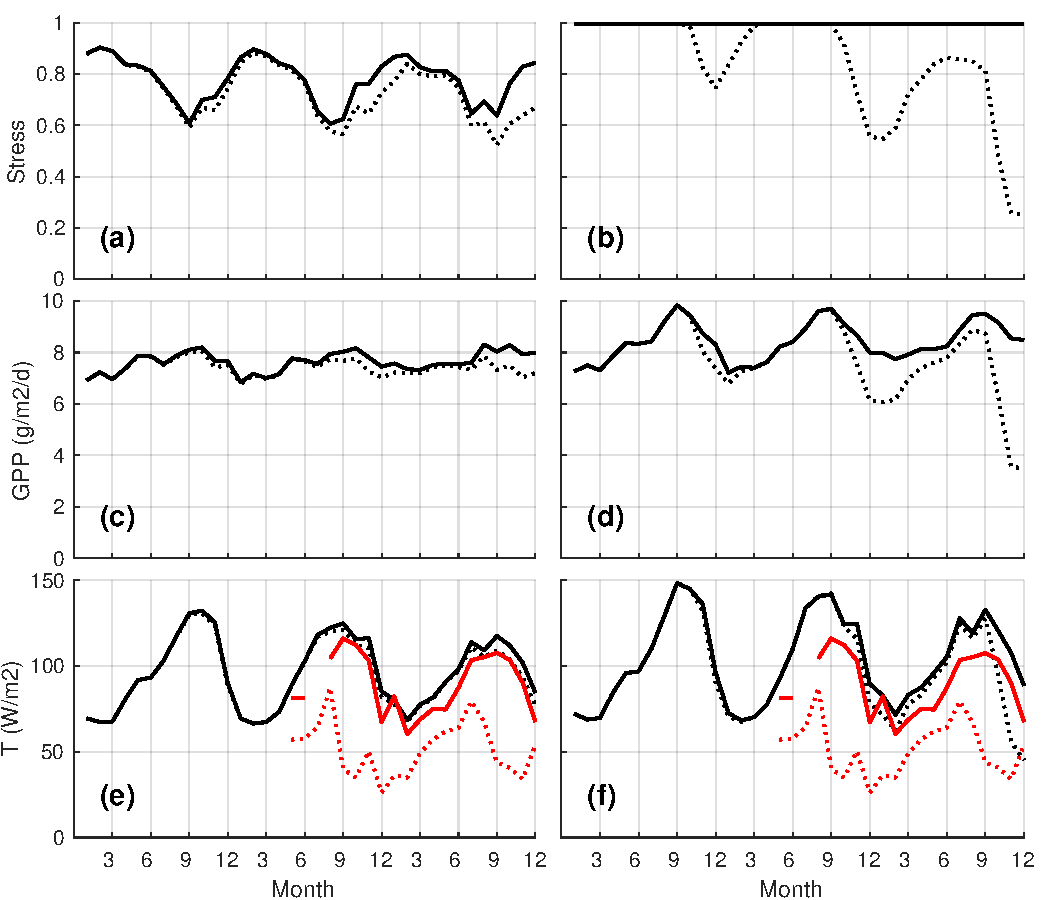
\includegraphics[width=30pc]{../figs/fig12.pdf}
     \caption{(a,b) Monthly mean water stress function. Note that the water stress function equals 1 when there is no stress and 0 when fully stressed.
     (c,d) Monthly mean transpiration (W/m$^2$).
     (e,f) Monthly mean gross primary productivity (g/m$^2$/d). 
     Solid lines correspond to ambient throughfall conditions, and dotted lines feature 50\% throughfall exclusion.
     Black lines represent model output.
     Red lines show observational transpiration derived from sap flux (see zqz).
     PHS is on for (a), (c), and (e). PHS is off for (b), (d), and (f).
     }
     \label{fig3a}
  \end{figure}
  
          \clearpage
    \begin{figure}[h]
     \centering
     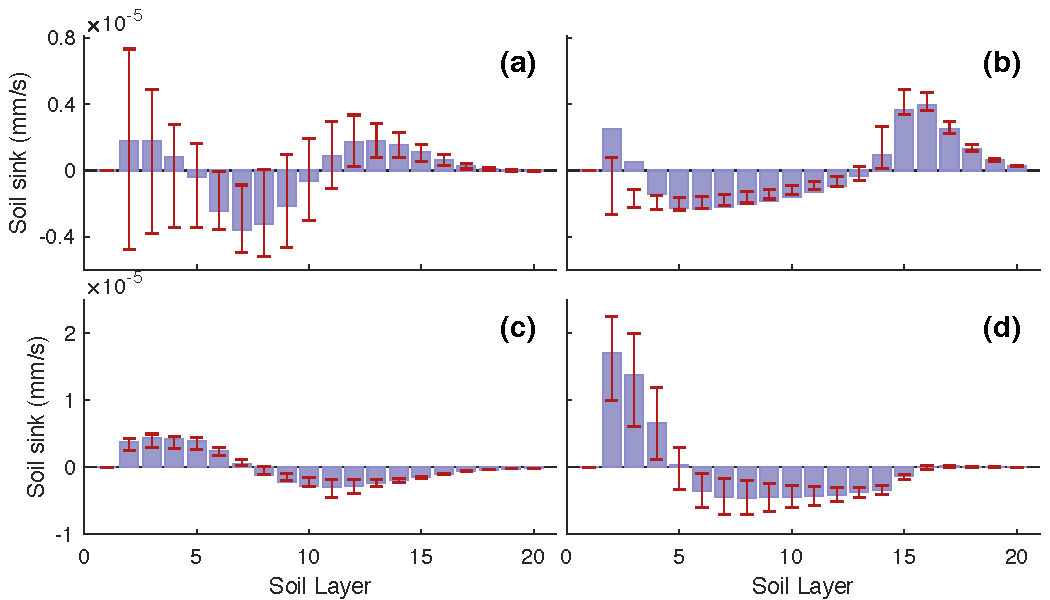
\includegraphics[width=30pc]{../figs/fig10.pdf}
     \caption{2003 Dry season (SON) diurnal mean water stress function for 
     (a) PHS on, and
     (b) PHS off.
     Solid lines correspond to ambient throughfall conditions, and dotted lines feature 50\% throughfall exclusion.
     }
     \label{fig2}
  \end{figure}
  
      \clearpage
    \begin{figure}[h]
     \centering
     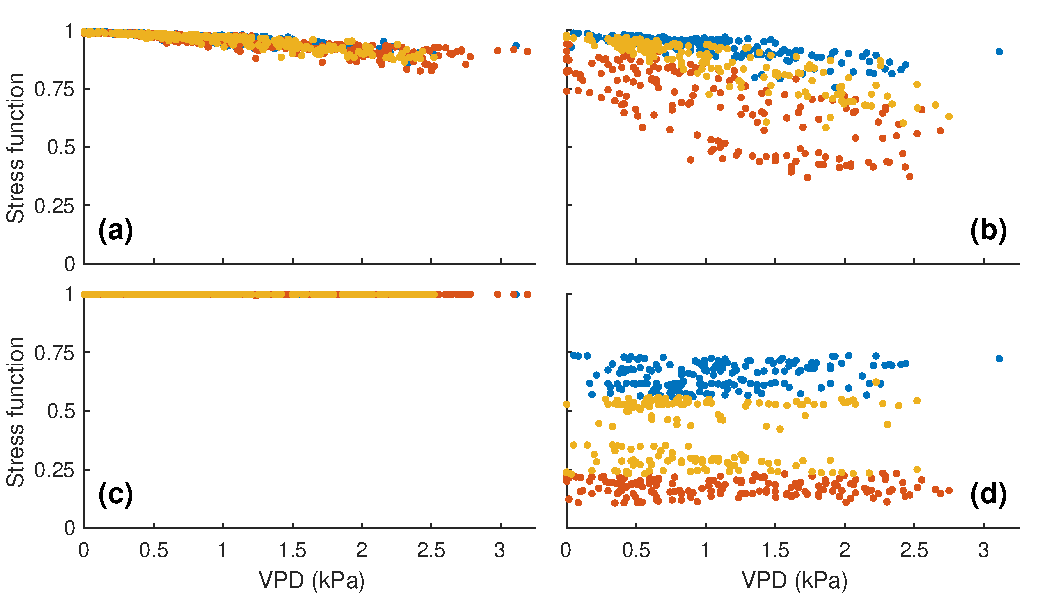
\includegraphics[width=30pc]{../figs/fig9.pdf}
     \caption{Water stress function versus vapor pressure deficit, for points with downwelling shortwave radiation between 400 and 425 W/m2.
     (a) PHS-on, ambient throughfall
     (b) PHS-on, 50\% throughfall excluded
     (c) PHS-off, ambient throughfall
     (d) PHS-off, 50\% throughfall excluded. 
     For (a) and (b) data are subdivided based on predawn root water potential.
     For (c) and (d) data are subdivided based on average soil matric potential, weighted by root fraction.
     Blue dots represent the highest tercile, yellow dots represent the intermediate tercile, and red dots represent the most negative tercile.
     }
     \label{fig5}
       \end{figure}
  
  
\clearpage   
  \begin{figure}[h]
     \centering
     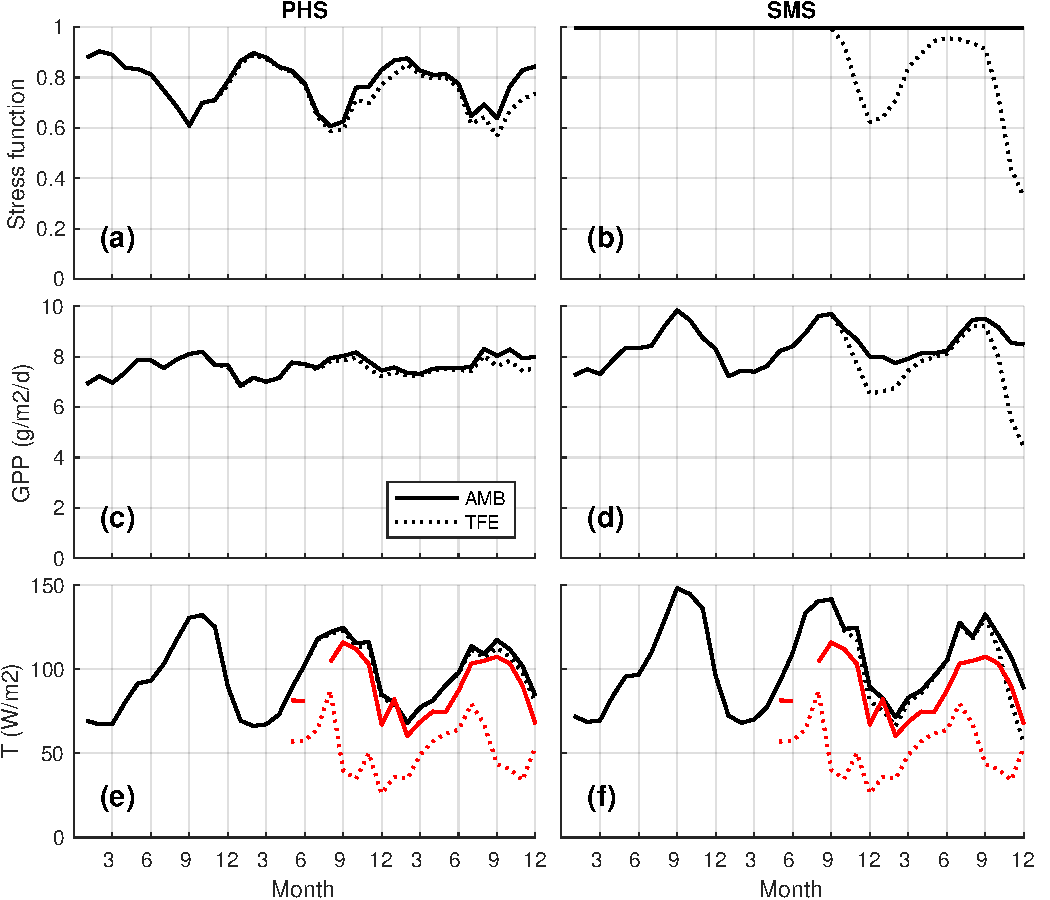
\includegraphics[width=30pc]{../figs/fig3.pdf}
     \caption{Distribution of daytime soil-to-root hydraulic conductance by soil layer. Bars span interquartile range and x's mark the median. 
     (a) PHS-on, ambient throughfall, all timesteps.
     (b) PHS-on, Jan 1, 2002 to Dec 31, 2003 with 50\% throughfall excluded.
     (c) PHS-off, ambient throughfall, all timesteps.
     (d) PHS-off, Jan 1, 2002 to Dec 31, 2003 with 50\% throughfall excluded.
     }
     \label{fig3a}
  \end{figure}
  \clearpage
    \begin{figure}[h]
     \centering
     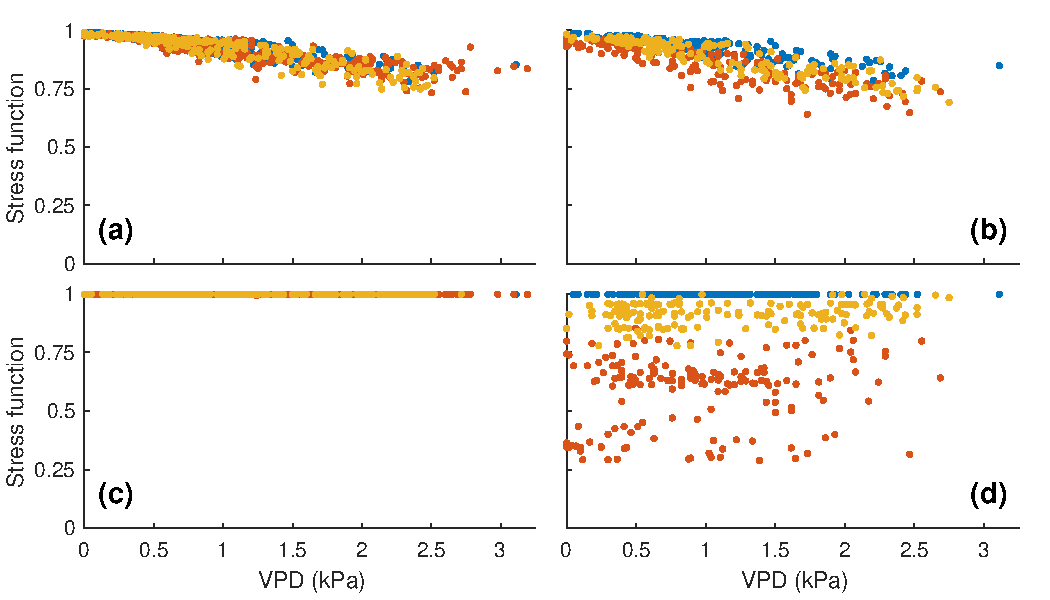
\includegraphics[width=30pc]{../figs/fig5.pdf}
     \caption{Total hydraulic redistribution (mm) by month over two years (2002-3). For (a) ambient throughfall conditions, and (b) 50\% throughfall exclusion.      }
     \label{fig2}
  \end{figure}
  
    \clearpage
    \begin{figure}[h]
     \centering
     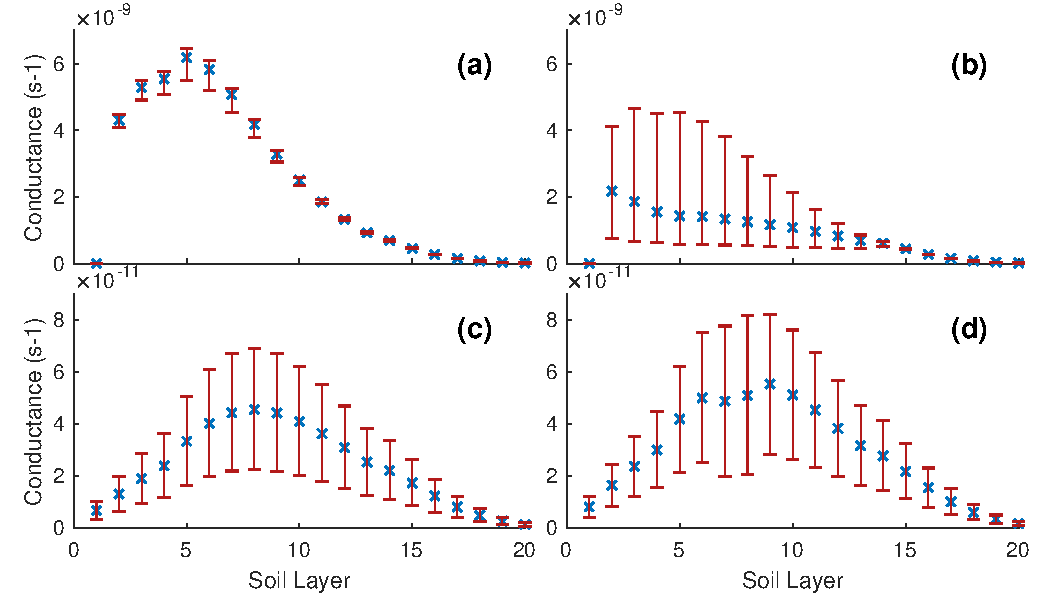
\includegraphics[width=30pc]{../figs/fig6.pdf}
     \caption{PHS-on, Nighttime (6pm to 6am)  soil sink by layer.
          Bars show mean and lines span interquartile range, for 
     (a) September 2001-3, ambient throughfall,
     (b) December 2001-3, ambient throughfall,
     (c) September 2002-3, 50\% throughfall excluded,
     (d) December 2002-3, 50\% throughfall excluded. 
     Note that positive values correspond to water extracted from the given soil layer, 
     and negative values correspond to water deposited into the given soil layer.}
     \label{fig2}
  \end{figure}
  
      \clearpage
    \begin{figure}[h]
     \centering
     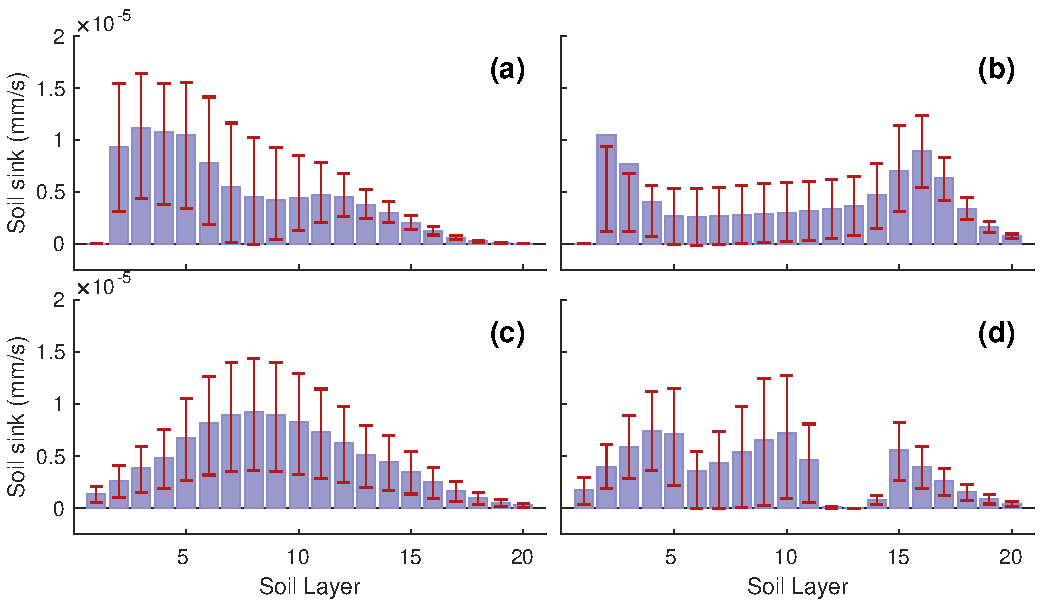
\includegraphics[width=30pc]{../figs/fig7.pdf}
     \caption{PHS-on, Daytime (6am to 6pm) soil sink by layer. 
     Bars show mean and lines span interquartile range, for 
     (a) September 2001-3, ambient throughfall,
     (b) December 2001-3, ambient throughfall,
     (c) September 2002-3, 50\% throughfall excluded,
     (d) December 2002-3, 50\% throughfall excluded. 
     Note that positive values correspond to water extracted from the given soil layer, 
     and negative values correspond to water deposited into the given soil layer.}
     \label{fig2}
  \end{figure}
  
        \clearpage
    \begin{figure}[h]
     \centering
     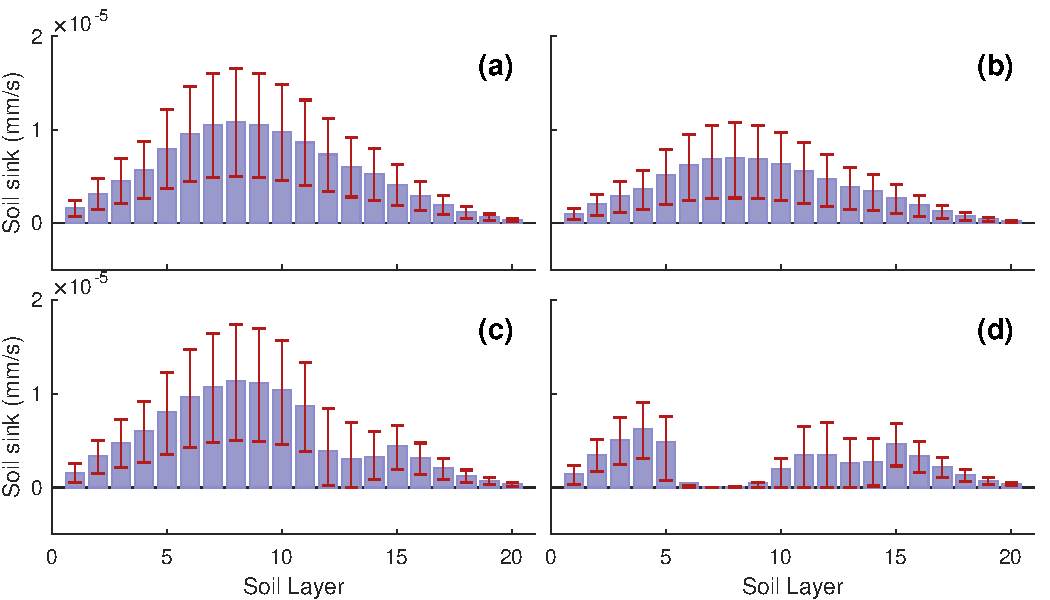
\includegraphics[width=30pc]{../figs/fig8.pdf}
     \caption{PHS-off, Daytime (6am to 6pm) soil sink by layer. 
          Bars show mean and lines span interquartile range, for  
     (a) September 2001-3, ambient throughfall,
     (b) December 2001-3, ambient throughfall,
     (c) September 2002-3, 50\% throughfall excluded,
     (d) December 2002-3, 50\% throughfall excluded. }
     \label{fig2}
  \end{figure}
  


  


\clearpage

\appendix
%====================
%  APPENDIX
%====================
\section{Appendix to Model Description}

% Details on water supply
\subsection{Details of Water Supply}

PHS resolves flow across four different segments, soil-to-root, root-to-stem, stem-to-leaf, and leaf-to-transpiration.

Stem-to-leaf. The area bases are sunlit and shaded leaf area, respectively. 
Note that gravity is assumed negligible here. 
Likewise there is no length scaling applied to maximum conductance. 
Therefore the input parameters for $k_{1,\text{max}}$ should be conductances ($s^{-1}$).

\begin{linenomath*} \begin{equation} \begin{aligned}
q_{1a} &= k_{1} \cdot \text{LAI-sun}  \cdot \left( \psi_{\text{stem}}-\psi_{\text{sun-leaf}}\right) \\
q_{1b} &= k_{1} \cdot \text{LAI-shade} \cdot  \left( \psi_{\text{stem}}-\psi_{\text{shade-leaf}}\right)
\end{aligned} \end{equation} \end{linenomath*}

\begin{linenomath*} \begin{equation}
k_{1} = k_{1,\text{max}} \cdot f\left(\psi_{\text{stem}}\right)
\end{equation} \end{linenomath*}

\begin{linenomath*} \begin{equation} \begin{aligned}
f\left(\psi\right)=2^{-\left(\dfrac{\psi}{p_{50}}\right)^{c_k}}
\end{aligned} \end{equation} \end{linenomath*}

Root-to-stem. The area basis is stem area index. 
The parameter is maximum stem xylem conductivity ($K_{2,\text{max}}$).
Stem conductance ($k_2$) is the result of scaling maximum conductivity by the tree height ($h$)
and applying loss relative to maximum conductance via the vulnerability curve $f\left(\psi_{\text{root}}\right)$. 
\begin{linenomath*} \begin{equation}
q_2 = k_2 \cdot  \text{SAI}  \cdot \left( \psi_{\text{root}}-\psi_{\text{stem}}-\rho g h\right)
\end{equation} \end{linenomath*}
\begin{linenomath*} \begin{equation}
k_2 = \dfrac{K_{2,\text{max}}}{h} \cdot f\left(\psi_{\text{root}}\right)
\end{equation} \end{linenomath*}

Soil-to-root. Area basis is RAI in soil layer $i$, which is based on the layer root fraction times the
total root area. Total root area we have as the summed stem and leaf area indices multiplied by a relative
root area parameter ($f_{\text{root}}$).
The vertical root distribution is defined by the layer root fraction ($r_i$), which follows a one-parameter 
(by PFT) power law decay following \citet{jackson1996}.

\begin{linenomath*} \begin{equation}
q_{3,i} = k_{3,i} \cdot  \text{RAI}_i  \cdot \left( \psi_{\text{soil,i}}-\psi_{\text{root}}-\rho g z_i\right)
\end{equation} \end{linenomath*}
\begin{linenomath*} \begin{equation}
\text{RAI}_i=f_{\text{root}} \cdot \left( \text{SAI} + \text{LAI} \right) \cdot r_i
\end{equation} \end{linenomath*}
\begin{linenomath*} \begin{equation}
k_{3,i} = \dfrac{k_{r,i}+k_{s,i}}{k_{r,i}\cdot k_{s,i}}
\end{equation} \end{linenomath*}
\begin{linenomath*} \begin{equation}
k_{r,i} = \dfrac{K_{r,\text{max}}}{l_i} f \left(\psi_{\text{soil,i}}\right)
\end{equation} \end{linenomath*}
\begin{linenomath*} \begin{equation}
l_i = z_i + x
\end{equation} \end{linenomath*}
\begin{linenomath*} \begin{equation}
k_{s,i} = \dfrac{K_{s,i}}{d}
\end{equation} \end{linenomath*}

The conductance $k_{3,i}$ reflects two resistors in series, from soil-to-root ($k_{s,i}$) and through the
root tissue ($k_{r,i}$).
The root tissue conductance is attenuated via the vulnerability curve framework. 
The input parameter is maximum root xylem conductivity, on the basis of RAI as defined above.
The root conductivity is scaled by the conducting length, which is estimated as the sum of soil layer depth ($z_i$)
and average lateral extent ($x$, static parameter).
The soil conductivity $K_{s,i}$ is calculated from the layer soil matric potential ($\psi_s$) 
and soil properties following \citet{clapp1978} as described in \citet{oleson2013}.
The soil conductance ($k_{s,i}$) is the result of scaling the conductivity by $d$, 
 the distance between roots estimated following \citet{williams1996} and \citet{bonan2014}

The challenge here is obviously getting your head around all the parameters.

% Details on water demand
\subsection{Details of Water Supply}

% Details on phs solution
\subsection{Details of Solution}


The continuity of water flow through the system yields four equations
   \begin{linenomath*} \begin{equation}
   \begin{aligned}
   E_{sun}&=q_{1a}\\
   E_{shade}&=q_{1b}\\
   q_{1a}+q_{1b}&=q_2\\
   q_2&=\sum_{i=1}^{nlevsoi}{q_{3,i}}
   \end{aligned}
   \end{equation} \end{linenomath*}

We seek the set of vegetation water potential values (four unknowns), 

   \begin{linenomath*} \begin{equation}
   \psi=\left[ \begin {array}{c} 
   \psi_{sunleaf}\cr\psi_{shadeleaf}\cr\psi_{stem}\cr\psi_{root}
   \end {array} \right] 
   \end{equation} \end{linenomath*}

that satisfies these equations, as forced by the soil moisture and atmospheric state. 

Each flux on the schematic can be represented in terms of the relevant water potentials. 

Defining the transpiration fluxes:


   \begin{linenomath*} \begin{equation}
   \begin{aligned}
   E_{sun} &= E_{sun,max} \cdot 2^{-\left(\dfrac{\psi_{sunleaf}}{p50_e}\right)^{c_k}} \\
   E_{shade} &= E_{shade,max} \cdot 2^{-\left(\dfrac{\psi_{shadeleaf}}{p50_e}\right)^{c_k}} 
   \end{aligned}
   \end{equation} \end{linenomath*}

Defining the water supply fluxes:

   \begin{linenomath*} \begin{equation}
   \begin{aligned}
   q_{1a}&=k_{1a,max}\cdot 2^{-\left(\dfrac{\psi_{stem}}{p50_1}\right)^{c_k}} \cdot\mbox{LAI}_{sun}\cdot\left(\psi_{stem}-\psi_{sunleaf} \right) \\
   q_{1b}&=k_{1b,max}\cdot 2^{-\left(\dfrac{\psi_{stem}}{p50_1}\right)^{c_k}}\cdot\mbox{LAI}_{shade}\cdot\left(\psi_{stem}-\psi_{shadeleaf} \right) \\
   q_2&=\dfrac{k_{2,max}}{z_2} \cdot 2^{-\left(\dfrac{\psi_{root}}{p50_2}\right)^{c_k}} \cdot SAI \cdot \left( \psi_{root} - \psi_{stem} - \Delta \psi_z  \right) \\
   q_{soil}&=\sum_{i=1}^{nlevsoi}{q_{3,i}}=\sum_{i=1}^{nlevsoi}{k_{3,i}\cdot RAI\cdot\left(\psi_{soil,i}-\psi_{root} + \Delta\psi_{z,i} \right)}
   \end{aligned}
   \end{equation} \end{linenomath*}

We're looking to find the vector $\psi$
that fits with soil and atmospheric forcings while satisfying water flow continuity. 
Due to the model non-linearity, we use a linearized explicit approach, iterating with Newton's method. 
The initial guess is the solution for $\psi$ (vector) from the previous time step. 
The general framework, from iteration $m$ to $m+1$ is:

   \begin{linenomath*} \begin{equation} 
   \begin{aligned}
   q^{m+1}&=q^m+\dfrac{\delta q}{\delta\psi}\Delta\psi \\
   \psi^{m+1}&=\psi^{m}+\Delta\psi
   \end{aligned}
   \end{equation} \end{linenomath*}

So for our first flux balance equation, at iteration $m+1$, we have:

   \begin{linenomath*} \begin{equation} 
   E_{sun}^{m+1}=q_{1a}^{m+1}
   \end{equation} \end{linenomath*}

Which can be linearized to:

   \begin{linenomath*} \begin{equation} 
   E_{sun}^{m}+\dfrac{\delta E_{sun}}{\delta\psi}\Delta\psi=q_{1a}^{m}+\dfrac{\delta q_{1a}}{\delta\psi}\Delta\psi
   \end{equation} \end{linenomath*}

And rearranged to be:

   \begin{linenomath*} \begin{equation} 
   \dfrac{\delta q_{1a}}{\delta\psi}\Delta\psi-\dfrac{\delta E_{sun}}{\delta\psi}\Delta\psi=E_{sun}^{m}-q_{1a}^{m}
   \end{equation} \end{linenomath*}

And for the other 3 flux balance equations:

   \begin{linenomath*} \begin{equation} 
   \begin{aligned}
   \dfrac{\delta q_{1b}}{\delta\psi}\Delta\psi-\dfrac{\delta E_{sha}}{\delta\psi}\Delta\psi&=E_{sha}^{m}-q_{1b}^{m} \\
   \dfrac{\delta q_2}{\delta\psi}\Delta\psi-\dfrac{\delta q_{1a}}{\delta\psi}\Delta\psi-\dfrac{\delta q_{1b}}{\delta\psi}\Delta\psi&=q_{1a}^{m}+q_{1b}^{m}-q_2^{m} \\
   \dfrac{\delta q_{soil}}{\delta\psi}\Delta\psi-\dfrac{\delta q_2}{\delta\psi}\Delta\psi&=q_2^{m}-q_{soil}^{m}
   \end{aligned}
   \end{equation} \end{linenomath*}

Putting all four together in matrix form:

   \begin{linenomath*} \begin{equation} 
   \left[ \begin {array}{c}
   \dfrac{\delta q_{1a}}{\delta\psi}-\dfrac{\delta E_{sun}}{\delta\psi} \cr
   \dfrac{\delta q_{1b}}{\delta\psi}-\dfrac{\delta E_{sha}}{\delta\psi} \cr
   \dfrac{\delta q_2}{\delta\psi}-\dfrac{\delta q_{1a}}{\delta\psi}-\dfrac{\delta q_{1b}}{\delta\psi} \cr
   \dfrac{\delta q_{soil}}{\delta\psi}-\dfrac{\delta q_2}{\delta\psi}
   \end {array} \right]
   \Delta\psi=
   \left[ \begin {array}{c}
   E_{sun}^{m}-q_{1a}^{m} \cr
   E_{sha}^{m}-q_{1b}^{m} \cr
   q_{1a}^{m}+q_{1b}^{m}-q_2^{m} \cr
   q_2^{m}-q_{soil}^{m}
   \end {array} \right]
   \end{equation} \end{linenomath*}

Now to expand the left-hand side, from vector $\psi$ to the four distinct plant water potential nodes, noting that many derivatives are zero (e.g. $\dfrac{\delta E_{sun}}{\delta\psi_{sha}}=0$)

Introducing the notation:
$A\Delta\psi=b$

   \begin{linenomath*} \begin{equation} 
   \Delta\psi=\left[ \begin {array}{c}
   \Delta\psi_{sunleaf} \cr
   \Delta\psi_{shadeleaf} \cr
   \Delta\psi_{stem} \cr
   \Delta\psi_{root}
   \end {array} \right] 
   \end{equation} \end{linenomath*}

   \begin{linenomath*} \begin{equation} 
   A=
   \left[ \begin {array}{cccc}
   \dfrac{\delta q_{1a}}{\delta \psi_{sun}}-\dfrac{\delta E_{sun}}{\delta \psi_{sun}}&0&\dfrac{\delta q_{1a}}{\delta \psi_{stem}}&0\cr
   0&\dfrac{\delta q_{1b}}{\delta \psi_{sha}}-\dfrac{\delta E_{sha}}{\delta \psi_{sha}}&\dfrac{\delta q_{1b}}{\delta \psi_{stem}}&0\cr
   -\dfrac{\delta q_{1a}}{\delta \psi_{sun}}&
   -\dfrac{\delta q_{1b}}{\delta \psi_{sha}}&
   \dfrac{\delta q_2}{\delta \psi_{stem}}-\dfrac{\delta q_{1a}}{\delta \psi_{stem}}-\dfrac{\delta q_{1b}}{\delta \psi_{stem}}&
   \dfrac{\delta q_2}{\delta \psi_{root}}\cr
   0&0&-\dfrac{\delta q_2}{\delta \psi_{stem}}&\dfrac{\delta q_{soil}}{\delta \psi_{root}}-\dfrac{\delta q_2}{\delta \psi_{root}}
   \end {array} \right]
   \end{equation} \end{linenomath*}

   \begin{linenomath*} \begin{equation} 
   b=
   \left[ \begin {array}{c}
   E_{sun}^{m}-q_{b1}^{m} \cr
   E_{sha}^{m}-q_{b2}^{m} \cr
   q_{b1}^{m}+q_{b2}^{m}-q_{stem}^{m} \cr
   q_{stem}^{m}-q_{soil}^{m}
   \end {array} \right]
   \end{equation} \end{linenomath*}

Now we compute all the entries for $A$ and $b$ based on the soil moisture and maximum transpiration forcings and can solve to find:

   \begin{linenomath*} \begin{equation} 
   \Delta\psi=A^{-1}b
   \end{equation} \end{linenomath*}

   \begin{linenomath*} \begin{equation} 
   \psi_{m+1}=\psi_m+\Delta\psi
   \end{equation} \end{linenomath*}

We iterate until $b\to 0$, signifying water flux balance through the system. The result is a final set of water potentials ( $\psi_{root}$, $\psi_{xylem}$, $\psi_{shadeleaf}$, $\psi_{sunleaf}$) satisfying non-divergent water flux through the system. 
The magnitude of the water flux is driven by soil matric potential and unstressed ( $\beta_t=1$) transpiration. 

We use the transpiration solution (corresponding to the final solution for $\psi$) to compute stomatal conductance. The stomatal conductance is then used to compute $\beta_t$. 

   \begin{linenomath*} \begin{equation} 
   \beta_{t,sun} = \dfrac{g_{s,sun}}{g_{s,sun,\beta_t=1}} 
   \end{equation} \end{linenomath*}

   \begin{linenomath*} \begin{equation} 
   \beta_{t,shade} = \dfrac{g_{s,shade}}{g_{s,shade,\beta_t=1}} 
   \end{equation} \end{linenomath*}

The $\beta_t$ values are used in the Photosynthesis module (see section \ref{sect:A}) to apply water stress. 
The solution for $\psi$ is saved as a new variable (vegetation water potential) and is indicative of plant water status.
The soil-to-root fluxes $\left( q_{3,1},q_{3,2},\text{...},q_{3,n}\right)$ are used as the soil transpiration sink in the Richards' equation subsurface flow equations.

\acknowledgments
 = enter acknowledgments here =


%====================
%   REFERENCES
%====================
\nocite{*} 
\bibliography{refs/all}


\listofchanges


\end{document}


